\documentclass[twoside]{amsart}
\usepackage{amssymb,latexsym}
\usepackage{xspace}
\usepackage{enumerate}
\usepackage{graphics}
\newcommand{\Rationals}{\mathbb{Q}{}}
\newcommand{\Reals}{\mathbb{R}{}}
\newcommand{\Integers}{\mathbb{Z}{}}
\newcommand{\Solution}{\textsc{Solution}\xspace}
\newcommand{\Problem}{\textsc{Problem}\xspace}
\newcommand{\Blank}{\mathrel{\phantom{=}}}
\newcommand{\ltrue}{\top}
\newcommand{\lfalse}{\bot}
\begin{document}
\title{Answers to Chapter 3 Exercises - A Book of Abstract Algebra}
\author{Michael Welch}
\date{\today}
\maketitle

This document contains selected answers to exercises from chapter 3
of A Book of Abstract Algebra.

\begin{enumerate}[A.]
   \item \textsc{Examples of Abelian Groups}

   Prove that each of the following sets, with the indicated operation, is an
   abelian group.

   \textbf{Instructions} Proceed as in Chapter 2, Exercise B.

   \begin{enumerate}[1.]
      \item $x * y = x + y + k$ (k is a fixed constant), on the set 
      $\Reals$ of the real numbers.

      \begin{enumerate} % 4 parts: assoc, commut, identity, inverse
	 \item 
	 \begin{proof}[Proof that operation is commutative]
	    \begin{align*}
	       x * y & = x + y + k \\
	       y * x & = y + x + k \\
		     & = x + y + k && \text{Commute addition} \qedhere
	    \end{align*}
	 \end{proof}

	 \item 
	 \begin{proof}[Proof that operation is associative]
	    \begin{align*}
	       x * (y * z) & = x * (y + z + k) \\
			   & = x + (y + z + k) + k \\
			   & = x + y + z + 2k \\
	       (x * y) * z & = (x + y + k) * z \\
			   & = (x + y + k) + z + k \\
			   & = x + y + z + 2k \qedhere
	    \end{align*}
	 \end{proof}

	 \item The identity element can be calculated:
	 \begin{align*}
	    x * e & = x         \\
	    x * e & = x + e + k \\
		x & = x + e + k \\
		e & = -k
	 \end{align*}

	 We know by commuativity that $x * (-k) = (-k) * x$. Therefore,
	 $-k$ is the identity element.

	 \item We can caluclate the inverse of $x$ which we label $x'$.
	 \begin{align*}
	    x * x' & = -k          \\
	    x * x' & = x + x' + k  \\
	       -k  & = x + x' + k  \\
		x' & = -x - 2k
	 \end{align*}

      \end{enumerate}

      \item $\displaystyle x * y = \frac{xy}{2}$, on the set $\{x \in \Reals
      : x \ne 0\}$
      
	 \begin{enumerate}
	    \item
	    \begin{proof}[Proof the operation is commutative]
	       \begin{align*}
		  x * y & = \frac{xy}{2}         \\
		  y * x & = \frac{yx}{2}         \\
			& = \frac{xy}{2} \qedhere
	       \end{align*}
	    \end{proof}

	    \item
	    \begin{proof}[Proof the operation is associative]
	       \begin{align*}
		  x * (y * z) & = x * \frac{yz}{2}   \\
			      & = \frac{x\displaystyle\frac{yz}{2}}{2} \\
			      & = \frac{xyz}{4} \\
		  (x * y) * z & = \frac{xy}{2} * z \\
			      & = \frac{\displaystyle \frac{xy}{2}z}{2} \\
			      & = \frac{xyz}{4} \qedhere
	       \end{align*}
	    \end{proof}

	    \item The following calculation shows that the identity element
	    is 2.
	    \begin{align*}
	       x * e & = x              \\
	       x * e & = \frac{xe}{2}   \\
		   x & = \frac{xe}{2}   \\
		   1 & = \frac{e}{2}    \\
		   e & = 2
	    \end{align*}

	    \item The following calculation shows that the inverse of
	    $x$ is $4/x$.
	    \begin{align*}
	       x * x' & = 2             \\
	       x * x' & = \frac{xx'}{2} \\
		   2  & = \frac{xx'}{2} \\
		   4  & = xx'           \\
		   x' & = 4/x    && \text{$x \ne 0$ is given}
	    \end{align*}
	 \end{enumerate}

	 \item $x * y = x + y + xy$, on the set $\{x \in \Reals : x \ne -1\}$
	 \begin{enumerate}
	    \item
	    \begin{proof}[Proof the operation is commutative]
	       \begin{align*}
		  x * y & = x + y + xy \\
		  y * x & = y + x + yx \\
			& = x + y + xy \qedhere
	       \end{align*}
	    \end{proof}

	    \item
	    \begin{proof}[Proof the operation is associative]
	       \begin{align*}
		  x * (y * z) & = x * (y + z + yz) \\
			      & = x + (y + z + yz) + x(y + z + yz) \\
			      & = x + y + z + yz + xy + xz + xyz\\
			      & = x + y + xy + xz + yz + xyz \\
		  (x * y) * z & = (x + y + xy) * z \\
			      & = (x + y + xy) + z + (x + y + xy)z \\
			      & = x + y + xy + z + xz + yz + xyz \\
			      & = x + y + xy + xz + yz + xyz \qedhere
	       \end{align*}
	    \end{proof}

	    \item The following calculation shows the identity element to
	    be 0.
	    \begin{align*}
	       x * e & = x           \\
	       x * e & = x + e + xe  \\
		   x & = x + e + xe  \\
		   0 & =     e + xe  \\
		   0 & =   e(1 + x)  \\
		   e & = 0 && \text{$x\ne-1$ given}
	    \end{align*}

	    \item The following calculation shows the inverse of $x$ is 
	    $\displaystyle \frac{-x}{1+x}$.
	    \begin{align*}
	       x * x' & = 0            \\
	       x * x' & = x + x' + xx' \\
		    0 & = x + x' + xx' \\
		    0 & = x + x'(1 + x) \\
		   -x & = x'(1+x) \\
	       x'(1+x)& = -x \\
		   x' & = \frac{-x}{1+x} && \text{$x\ne-1$ given}
	    \end{align*}

	 \end{enumerate}

	 \item $x * y = \displaystyle \frac{x + y}{xy + 1}$, on the set
	 $\{x \in \Reals : -1 < x < 1\}$.
	 \begin{enumerate}
	    \item
	    \begin{proof}[Proof the operation is commutative]
	       \begin{align*}
		  x * y & = \frac{x+y}{xy + 1} \\
		  y * x & = \frac{y+x}{yx + 1} \\
			& = \frac{x+y}{xy + 1} \qedhere
	       \end{align*}
	    \end{proof}

	    \item
	    \begin{proof}[Proof the operation is associative]
	       \begin{align*}
		  x * (y * z) & = x * \frac{y + z}{yz + 1} \\
			      & = \frac{x + \displaystyle \frac{y + z}{yz + 1}}
				  {x\displaystyle \frac{y + z}{yz + 1} + 1} \\
			      & = \frac{x(yz+1)+y+z}{xy+xz+yz+1} \\
			      & = \frac{x + y + z + xyz}{xy + xz + yz + 1}
				  \qedhere
	       \end{align*}
	    \end{proof}

	    \item The following caluclation shows the identity element to be 0.
	    \begin{align*}
	       x * e & = x \\
	       x * e & = \frac{x + e}{xe + 1} \\
		   x & = \frac{x + e}{xe + 1} \\
	       x + e & = x(xe + 1) \\
	       x + e & = x^2e + x \\
	       e - x^2e & = 0  \\
	       e(1-x^2) & = 0    \\
		   e & = 0  && \text{$-1 < x < 1$ is given}
	    \end{align*}

	    \item The following caluclation shows the inverse of $x$ to be
	    $-x$.
	    \begin{align*}
	       x * x' & = 0                      \\
	       x * x' & = \frac{x + x'}{xx' + 1} \\
		   0  & = \frac{x + x'}{xx' + 1} \\
		   0  & = x + x' \\
		   x' & = -x
	    \end{align*}
	 \end{enumerate}
   \end{enumerate}

   \item \textsc{Groups on the Set $\Reals \times \Reals$}

   The symbol $\Reals \times \Reals$ represents the set of all ordered pairs
   $(x,y)$ of real numbers.  $\Reals \times \Reals$ may therefore be identified
   with the set of all the points in the plane.  Which of the following subsets
   of $\Reals \times \Reals$, with the indicated operation, is a group?  Which
   is an abelian group?

   \textbf{Instructions} Proceed as in the preceding exercise. To find the
   identity element, which in these problems is an ordered pair $(e_1, e_2)$ of
   real numbers, solve the equation $(a,b) * (e_1, e_2) = (a,b)$ for $e_1$ and
   $e_2$. To find the inverse $(a',b')$ of $(a,b)$, solve the equation
   $(a,b)*(a',b')=(e_1,e_2)$ for $a'$ and $b'$. [Remember that $(x,y)=(x',y')$
   if and only if $x=x'$ and $y=y'$.]

      \begin{enumerate}[1.]
	 \item $(a,b)*(c,d)=(ad+bc,bd)$, on the set $\{(x,y) \in \Reals
	 \times \Reals : y \ne 0\}$.
	 \begin{enumerate}
	    \item The operation is commutative.
	    \begin{proof}
	       \begin{align*}
		  (a,b)*(c,d) & = (ad+bc,bd) \\
		  (c,d)*(a,b) & = (cb+da,db) \\
			      & = (ad+bc,bd) \qedhere
	       \end{align*}
	    \end{proof}

	    \item The operation is associative.
	    \begin{proof}
	       \begin{align*}
		  (a,b) * ((c,d) * (e,f)) & = (a,b) * (cf+de,df)  \\
					  & = (adf + b(cf+de), bdf) \\
					  & = (adf +bcf + bde, bdf) \\
		  ((a,b) * (c,d)) * (e,f) & = (ad+bc,bd) * (e,f)    \\
					  & = ((ad+bc)f+bde, bdf)   \\
					  & = (adf+bcf+bde,bdf) \qedhere
	       \end{align*}
	    \end{proof}

	    \item 
	    \begin{align*}
	       (a,b) * (e_1,e_2) & = (a,b)            \\
	       (a,b) * (e_1,e_2) & = (ae_2+be_1,be_2) \\
		       (a,b)     & = (ae_2+be_1,be_2) 
	    \end{align*}
	    This implies that $a=ae_2+be_1$ and $b=be_2$. So $e_2=1$
	    and $e_1=0$. So the identity element is $(0,1)$.

	    \item
	    \begin{align*}
	       (a,b) * (a',b') & = (0,1) \\
	       (a,b) * (a',b') & = (ab'+ba',bb') \\
		 (ab'+ba',bb') & = (0,1) \\
	    \end{align*}
	    This implies $ab'+ba'=0$ and $bb'=1$. So $b'=1/b$. Let's
	    solve for $a$:
	    \begin{align*}
	       ab'+ba' & = 0         \\
	       a(1/b) + ba' & = 0    \\
		    ba' & = -1(a/b)  \\
		    a' & = -a/b^2
	    \end{align*}
	    So $(a',b') = (-a/b^2,1/b)$. 

	 \end{enumerate}
      \end{enumerate} 
   \item \textsc{Groups of Subsets of a Set}

   If $A$ and $B$ are any two sets, their \emph{symmetric difference}
   is the set $A \ominus B$ defined as follows (see figure~\ref{fig:symmdif}):
   \begin{center}
   $$ A\ominus B = (A-B) \cup (B-A) $$
   \end{center}

   \textsc{Note}: $A - B$ represents the set obtained by removing from
   $A$ all the elements which are in $B$.

   \begin{figure}[ht]
      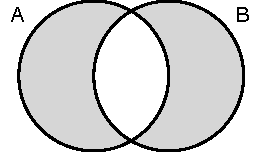
\includegraphics{img/symdiff.pdf}
      \caption{The shaded area is $A \ominus B$}
      \label{fig:symmdif}
   \end{figure}

   It is perfectly clear that $A \ominus B = B \ominus A$; hence this 
   operation is commutative. It is also associative, as the accompanying
   pictorial representation suggests: Let the union of $A$, $B$, and
   $C$ be divided into seven regions as illustrated.

   \begin{figure}[ht]
      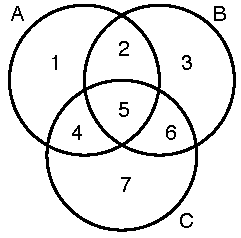
\includegraphics{img/symdiff3.pdf}
   \end{figure}

   \begin{gather*}
      A \ominus B \text{ consists of the regions 1, 4, 3, and 6.} \\
      B \ominus C \text{ consists of the regions 2, 3, 4, and 7.} \\
      A \ominus (B \ominus C) \text{ consists of the regions 1, 3, 5, and 7.}
      \\
      (A \ominus B) \ominus C \text{ consists of the regions 1, 3, 5, and 7.} 
   \end{gather*}

   \noindent Thus, $A \ominus (B \ominus C) = (A \ominus B) \ominus C$.


   If $D$ is a set, then the \emph{power set} of $D$ is the set $P_D$
   of all the subsets of $D$. That is,
   \begin{center}
   $$ P_D = \{ A : A \subseteq D \} $$
   \end{center}

   The operation $\ominus$ is to be regarded as an operation on $P_D$.

   \begin{enumerate}[1.]

   \item Prove that there is an identity element with respect to the operation
   $\ominus$. 

   \begin{proof}
   The identity element of $\ominus$ is $\emptyset$. 
   \begin{align*}
      A \ominus \emptyset & = (A - \emptyset) \cup (\emptyset - A) \\
                          & = A \cup \emptyset \\
			  & = A
   \end{align*}
   By inspection, it's obvious that $\ominus$ is commutative. Therefore,
   $\emptyset$ is the identity element.
   \end{proof}

   \item Prove every subset $A$ of $D$ has an inverse with respect to 
   $\ominus$, thus showing $\langle P_D,\ominus \rangle$ is a group!

   \begin{proof}
      The inverse of $A$ is $A$.
      \begin{align*}
         A \ominus A & = (A - A) \cup (A - A) \\
	             & = \emptyset \cup \emptyset \\
		     & = \emptyset
      \end{align*}
   \end{proof}

   \item Let $D$ be the three-element set $D = \{a,b,c\}$. List the elements
   of $P_D$. (For example, one element is $\{a\}$, another is $\{a,b\}$ and 
   so on. Do not forget the empty set and the whole set $D$.) Then
   write the operation table for $\langle P_D,\ominus \rangle$.

   \begin{center}
      $$ P_D = \{ \emptyset, \{a\}, \{b\}, \{c\}, \{a,b\}, \{b,c\}, 
                  \{a,c\}, \{a,b,c\} \} $$
   \end{center}

   \begin{center}
   \scalebox{.9}
   {\begin{tabular}{c|cccccccc}
      $\ominus$ & $\emptyset$ & $\{a\}$ & $\{b\}$ & $\{c\}$ & $\{a,b\}$ & 
          $\{b,c\}$ & $\{a,c\}$ & $\{a,b,c\}$  \\ \hline
      $\emptyset$ & $\emptyset$ & $\emptyset$ & $\emptyset$ & $\emptyset$ 
                  & $\emptyset$ & $\emptyset$ & $\emptyset$ & $\emptyset$\\
      $\{a\}$ & $\emptyset$ & $\emptyset$ & $\{a,b\}$ & $\{a,c\}$ & $\{b\}$ &
         $\{a,b,c\}$ & $\{c\}$ & $\{b,c\}$\\
      $\{b\}$ & $\emptyset$ & $\{a,b\}$ & $\emptyset$ & $\{b,c\}$ & $\{a\}$ &
         $\{c\}$ & $\{a,b,c\}$ & $\{a,c\}$ \\
      $\{c\}$ & $\emptyset$ & $\{a,c\}$ & $\{b,c\}$ & $\emptyset$ 
         & $\{a,b,c\}$ & $\{b\}$ & $\{a\}$ & $\{a,b\}$ \\
      $\{a,b\}$ & $\emptyset$ & $\{b\}$ & $\{a\}$ & $\{a,b,c\}$ & $\emptyset$ 
         & $\{a,c\}$ & $\{b,c\}$ & $\{c\}$ \\
      $\{a,c\}$ & $\emptyset$ & $\{c\}$ & $\{a,b,c\}$ & $\{a\}$ & $\{b,c\}$ 
         & $\{a,b\}$ & $\emptyset$ & $\{b\}$\\
      $\{b,c\}$ & $\emptyset$ & $\{a,b,c\}$ & $\{c\}$ & $\{b\}$ & $\{a,c\}$
         & $\emptyset$ & $\{a,b\}$ & $\{a\}$ \\
      $\{a,b,c\}$ & $\emptyset$ & $\{b,c\}$ & $\{a,c\}$ & $\{a,b\}$ & $\{c\}$ 
         & $\{a\}$ & $\{b\}$ & $\emptyset$\\
   \end{tabular}}
   \end{center}
   
   \begin{verbatim}

   \end{verbatim}

   \end{enumerate}

   \item \textsc{A Checkerboard Game}
      \begin{figure}[ht]
      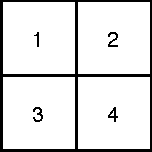
\includegraphics{img/checker.pdf}
   \end{figure}

   \noindent Our checkerboard has only four squares, numbered 1, 2, 3, and 4.
   There is a single checker on the board, and it has four possible moves:

   \begin{enumerate}
      \item[V:] Move vertically; that is, move from 1 to 3, or from 3 to 1, or
      from 2 to 4, or from 4 to 2. 
      \item[H:] Move horizontally; that is, move from 1 to 2 or vice versa,
      or from 3 to 4 or vice versa.
      \item[D:] Move diagonally; that is, move from 2 to 3 or vice versa, or
      move from 1 to 4 or vice versa.
      \item[I:] Stay put.
   \end{enumerate}

   \noindent We may consider an operation on the set of these four moves, which
   consists of performing moves successively. For example, if we move
   horizontally and then vertically, we end up with the same result as if we
   had moved diagonally:

   \begin{gather*}
      H * V = D
   \end{gather*}

   \noindent If we perform two horizontal moves in succession, we end up where
   we started: $H*H=I$. And so on. If $G=\{V,D,H,I\}$, and $*$ is the operation
   we have just described, write the table of $G$.

   \begin{center}
   \begin{tabular}{c|cccc}
      $*$ & $I$ & $V$ & $H$ & $D$ \\ \hline
      $I$ & $I$ & $V$ & $H$ & $D$ \\
      $V$ & $V$ & $I$ & $D$ & $H$ \\
      $H$ & $H$ & $D$ & $I$ & $V$ \\
      $D$ & $D$ & $H$ & $V$ & $I$
   \end{tabular}
   \end{center}
   
   \noindent Granting associativity, explain why $\langle G,* \rangle$ is a
   group.

   \emph{Explanation} $\langle G,* \rangle$ is a group because
   it has an identity element, $I$, and has an inverse for each element.
   We can see that for every element $M \in G$, $M * I = I * M = M$.
   Also, for every element $M$ we have an inverse $M^{-1} = M$.

   

   \item \textsc{A Coin Game}

   \item \textsc{Groups in Binary Codes}

   \item \textsc{Theory of Coding: Maximum Likelihood Decoding}

      \noindent 1.Verify
      
      \noindent 2. Let
      
      \noindent 3. Design
      
      \noindent 4. Decode

      In the remaining exercises, let $C$ be a code in $\mathbb{B}^n$,
      let $m$ denote the minimum distance in $C$, and let 
      $\mathbf{a}$ and $\mathbf{b}$ denote codewords in $C$.

      \noindent 5. Prove that it is possible to detect up to $m-1$ errors.
      (That is, if there are errors of transmission in $m-1$ or 
      fewer positions of a codeword, it can always be determined
      that the received word is incorrect.)

      \begin{proof}
	 Let $w$ be the sent word and $w'$ be the received word. Let 
	 $n$ be the number of errors in $w'$ such that $0 < n <= m - 1$. 
	 Assume that $w'$ is not determined to be incorrect. This means
	 that it was accepted as a codeword. However, the distance
	 between $w$ and $w'$ is $n$ and $n < m$. Therefore, the 
	 minimum distance of $C$ is $n$. But this contradicts
	 the definition of our code that states that $m$ is the minimum
	 distance. Therefore, our assumption is proved incorect, and
	 the word $w'$ will be detected to have errors.
      \end{proof}

      \noindent 6. By the \emph{sphere of radius} $k$ about a codeword
      $\mathbf{a}$ we mean the set of all words in $\mathbb{B}^n$
      whose distance from $\mathbf{a}$ is no greater than $k$. This set
      is denoted by $S_k(\mathbf{a})$; hence 
      \begin{center}
      $$ S_k(\mathbf{a}) = \{\mathbf{x} : d(\mathbf{a},\mathbf{x}) \le k \}$$
      \end{center}

      If $t=\frac{1}{2}(m-1)$, prove that any two spheres of radius $t$,
      say $S_t(\mathbf{a})$ and $S_t(\mathbf{b})$, have no elements in
      common. [\textsc{Hint}: Assume there is a word $\mathbf{x}$ such
      that $\mathbf{x} \in S_t(\mathbf{a})$ and $\mathbf{x}\in S_t(
      \mathbf{b})$. Using the definitions of $t$ and $m$, show that
      this is impossible.]

      \begin{proof}
         Assume there is a word $\mathbf{x}$ such that $\mathbf{x} \in
         S_t(\mathbf{a})$ and $\mathbf{x}\in S_t( \mathbf{b})$. 
	 This means that we need to flip at most $\frac{1}{2}(m-1)$ bits
	 to transform $\mathbf{a}$ into $\mathbf{x}$, and at most
	 $\frac{1}{2}(m-1)$ bits to tranform $\mathbf{x}$ into $\mathbf{b}$.
	 This implies that we need to flip at most 
	 $\frac{1}{2}(m-1) \times 2 = (m-1)$ bits to transform
	 $\mathbf{a}$ into $\mathbf{b}$. However, we know that the 
	 minimum distance between any two codewords is $m$. Therefore,
	 our assumption that $\mathbf{x}$ exists is false and there is
	 no common element between $S_t(\mathbf{a})$ and $S_t(\mathbf{b})$.
      \end{proof}

\end{enumerate}
\end{document}
